\documentclass[a4paper, 11pt]{article}
\usepackage{amsmath}
\usepackage{graphicx}
\usepackage{geometry}
\geometry{scale=0.8}
\linespread{1.5}
\usepackage{hyperref}
\usepackage{listings}
\usepackage{color}
\definecolor{dkgreen}{rgb}{0,0.6,0}
\definecolor{gray}{rgb}{0.5,0.5,0.5}
\definecolor{mauve}{rgb}{0.58,0,0.82}
\lstset{frame=shadowbox,
    language=python,
    aboveskip=3mm,
    belowskip=3mm,
    showstringspaces=false,
    columns=flexible,
    basicstyle={\small\ttfamily},
    keywordstyle=\color{blue},
    commentstyle=\color{dkgreen},
    stringstyle=\color{mauve},
    breaklines=true,
    breakatwhitespace=true,
    tabsize=3,
    numbers=left
}

\title{	
\normalfont \normalsize
\textsc{School of Data and Computer Science, Sun Yat-sen University} \\ [25pt] %textsc small capital letters
\rule{\textwidth}{0.5pt} \\[0.4cm] % Thin top horizontal rule
\huge  E09 Bayesian Network \\ % The assignment title
\rule{\textwidth}{2pt} \\[0.5cm] % Thick bottom horizontal rule
\author{17341203 Yixin Zhang}
\date{\normalsize\today}
}

\begin{document}
\maketitle
\tableofcontents
\newpage
\section{Pomegranate Installation}
\textbf{Under Linux:}
\begin{enumerate}
\item Install \texttt{python} first (\textbf{python 2}, not python 3).
\item Run \texttt{sudo apt-get install python-pip} to install \texttt{pip}.
\item Run \texttt{sudo pip install pomegranate} to install \texttt{pomegranate}.
\end{enumerate}
\begin{figure}[h]
  \centering
  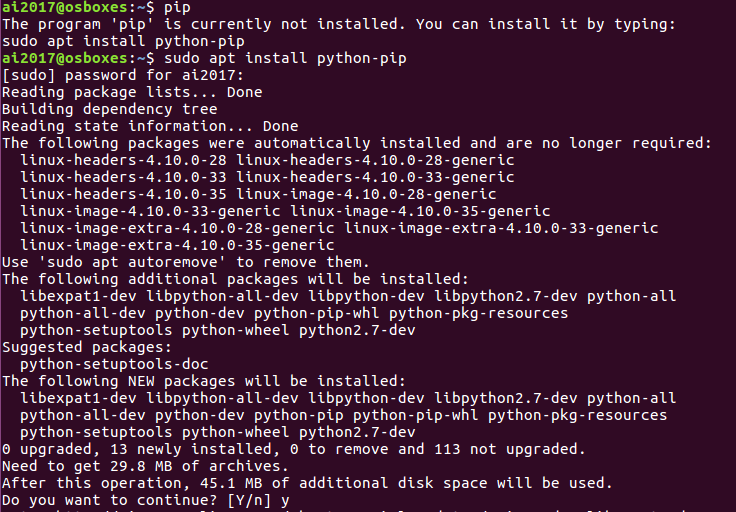
\includegraphics[width=7.5cm]{Pic/install1}
  \qquad
  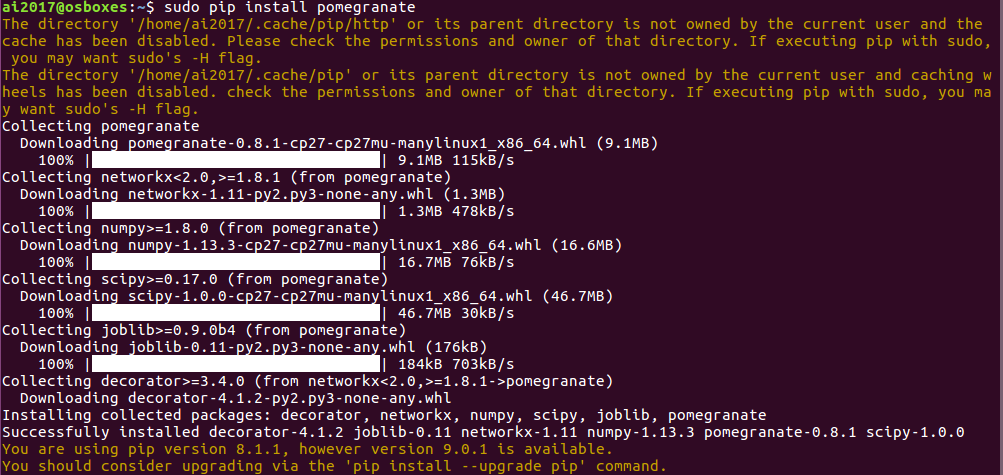
\includegraphics[width=8cm]{Pic/install2}
\end{figure}
\textbf{Under Windows}

You can also run \texttt{pip install pomegranate} if you have installed \texttt{pip}. If you don't know how to install \texttt{pip}, please click \url{https://jingyan.baidu.com/article/e73e26c0d94e0524adb6a7ff.html}.

For more, please click the homepage of Pomegranate - \url{https://github.com/jmschrei/pomegranate} for help. 
\begin{figure}[h]

  
  \centering
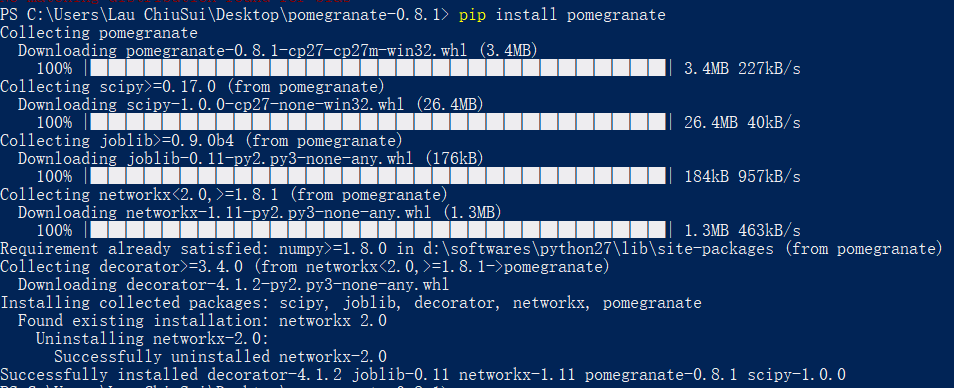
\includegraphics[width=16cm]{Pic/po}
  
\end{figure}

\section{Building Bayesian Network}
\label{sec:build-bayes-netw}
Please refer to \texttt{Tutorial\_4\_Bayesian\_Networks.pdf}. I will explain it in class.

\section{Tasks}
\label{sec:tasks}

\subsection{Burglary}
\label{sec:burglary}
\begin{figure}[h]
  \centering

  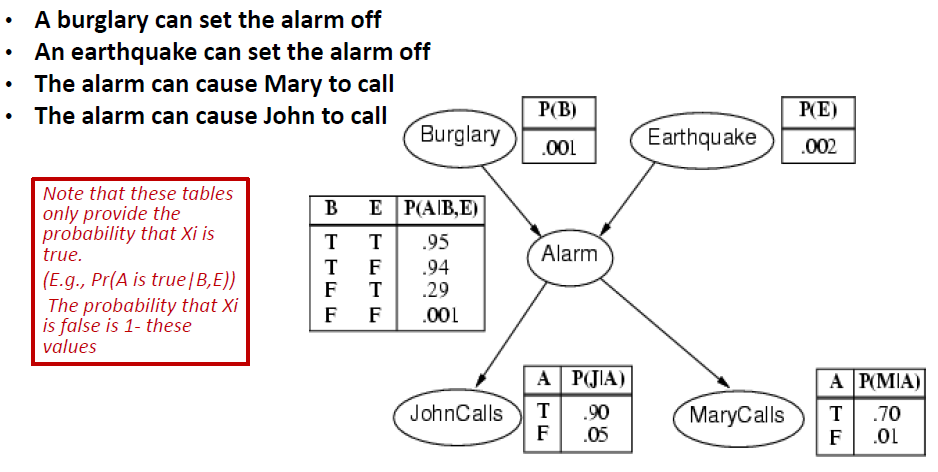
\includegraphics[width=14cm]{Pic/burglary}
\end{figure}
Please code to calculate:
\begin{enumerate}
\item $P(A)$
\item $P(J\overline{M})$
\item $P(A | J\overline{M})$
\item $P(B | A)$
  \item $P(B | J\overline{M})$
  \item  $P(J\overline{M} | \overline{B})$
\end{enumerate}
\begin{figure}[ht]
\centering
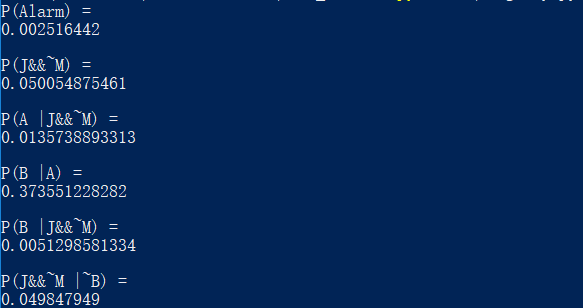
\includegraphics[width=12cm]{Pic/burglar_result}
\end{figure}
\subsection{Diagnosing}
\label{sec:bayesian-networks}
\textbf{Variables and their domais}
\begin{lstlisting}{language=Python}
(1)PatientAge:['0-30','31-65','65+']
(2)CTScanResult:['Ischemic Stroke','Hemmorraghic Stroke']
(3)MRIScanResult: ['Ischemic Stroke','Hemmorraghic Stroke']
(4)StrokeType: ['Ischemic Stroke','Hemmorraghic Stroke', 'Stroke Mimic']
(5)Anticoagulants: ['Used','Not used']
(6)Mortality:['True', 'False']
(7)Disability: ['Negligible', 'Moderate', 'Severe']
\end{lstlisting}
\textbf{CPTs}

\textbf{Note:} [CTScanResult, MRIScanResult,StrokeType] means:

P(StrokeType='...' $|$ CTScanResult='...' $\land$  MRIScanResult='...') 
\begin{lstlisting}{language=Python}
(1)
[PatientAge]

['0-30', 0.10],
['31-65', 0.30],
['65+', 0.60]

(2)
[CTScanResult]

['Ischemic Stroke',0.7],
[ 'Hemmorraghic Stroke',0.3]

(3)
[MRIScanResult]

['Ischemic Stroke',0.7],
[ 'Hemmorraghic Stroke',0.3]

(4)
[Anticoagulants]

[Used',0.5],
['Not used',0.5]

(5)
[CTScanResult, MRIScanResult,StrokeType])

['Ischemic Stroke','Ischemic Stroke','Ischemic Stroke',0.8],
['Ischemic Stroke','Hemmorraghic Stroke','Ischemic Stroke',0.5],  
[ 'Hemmorraghic Stroke','Ischemic Stroke','Ischemic Stroke',0.5],
[ 'Hemmorraghic Stroke','Hemmorraghic Stroke','Ischemic Stroke',0], 

['Ischemic Stroke','Ischemic Stroke','Hemmorraghic Stroke',0],
['Ischemic Stroke','Hemmorraghic Stroke','Hemmorraghic Stroke',0.4], 
[ 'Hemmorraghic Stroke','Ischemic Stroke','Hemmorraghic Stroke',0.4],
[ 'Hemmorraghic Stroke','Hemmorraghic Stroke','Hemmorraghic Stroke',0.9],

['Ischemic Stroke','Ischemic Stroke','Stroke Mimic',0.2],
['Ischemic Stroke','Hemmorraghic Stroke','Stroke Mimic',0.1],    
[ 'Hemmorraghic Stroke','Ischemic Stroke','Stroke Mimic',0.1],
[ 'Hemmorraghic Stroke','Hemmorraghic Stroke','Stroke Mimic',0.1],

(6) 
[StrokeType, Anticoagulants, Mortality]

['Ischemic Stroke', 'Used', 'False',0.28],
['Hemmorraghic Stroke', 'Used', 'False',0.99],
['Stroke Mimic', 'Used', 'False',0.1],
['Ischemic Stroke','Not used', 'False',0.56],
['Hemmorraghic Stroke', 'Not used', 'False',0.58],
['Stroke Mimic', 'Not used', 'False',0.05],

['Ischemic Stroke',  'Used' ,'True',0.72],
['Hemmorraghic Stroke', 'Used', 'True',0.01],
['Stroke Mimic', 'Used', 'True',0.9],
['Ischemic Stroke',  'Not used' ,'True',0.44],
['Hemmorraghic Stroke', 'Not used', 'True',0.42 ],
['Stroke Mimic', 'Not used', 'True',0.95]

(7)
[StrokeType, PatientAge, Disability]

['Ischemic Stroke',   '0-30','Negligible', 0.80],
['Hemmorraghic Stroke', '0-30','Negligible', 0.70],
['Stroke Mimic',        '0-30', 'Negligible',0.9],
['Ischemic Stroke',     '31-65','Negligible', 0.60],
['Hemmorraghic Stroke', '31-65','Negligible', 0.50],
['Stroke Mimic',        '31-65', 'Negligible',0.4],
['Ischemic Stroke',     '65+'  , 'Negligible',0.30],
['Hemmorraghic Stroke', '65+'  , 'Negligible',0.20],
['Stroke Mimic',        '65+'  , 'Negligible',0.1],

['Ischemic Stroke',     '0-30' ,'Moderate',0.1],
['Hemmorraghic Stroke', '0-30' ,'Moderate',0.2],
['Stroke Mimic',        '0-30' ,'Moderate',0.05],
['Ischemic Stroke',     '31-65','Moderate',0.3],
['Hemmorraghic Stroke', '31-65','Moderate',0.4],
['Stroke Mimic',        '31-65','Moderate',0.3],
['Ischemic Stroke',     '65+'  ,'Moderate',0.4],
['Hemmorraghic Stroke', '65+'  ,'Moderate',0.2],
['Stroke Mimic',        '65+'  ,'Moderate',0.1],

['Ischemic Stroke',     '0-30' ,'Severe',0.1],
['Hemmorraghic Stroke', '0-30' ,'Severe',0.1],
['Stroke Mimic',        '0-30' ,'Severe',0.05],
['Ischemic Stroke',     '31-65','Severe',0.1],
['Hemmorraghic Stroke', '31-65','Severe',0.1],
['Stroke Mimic',        '31-65','Severe',0.3],
['Ischemic Stroke',     '65+'  ,'Severe',0.3],
['Hemmorraghic Stroke', '65+'  ,'Severe',0.6],
['Stroke Mimic',        '65+'  ,'Severe',0.8]
\end{lstlisting}
\textbf{Calculation}

Please code to calculate the following probability value:

p1 = P(Mortality='True' $|$ PatientAge='31-65' $\land$ CTScanResult='Ischemic Stroke')

p2 = P(Disability='Moderate' $|$ PatientAge='65+' $\land$  MRIScanResult='Hemmorraghic Stroke')

p3 = P(StrokeType='Stroke Mimic' $|$ PatientAge='65+' $\land$ CTScanResult='Hemmorraghic Stroke' $\land$ MRIScanResult='Ischemic Stroke')

p4 = P(Anticoagulants='Not used' $|$ PatientAge='0-30')

\begin{figure}[ht]
\centering
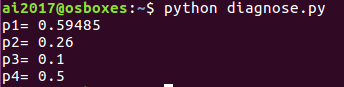
\includegraphics[width=12cm]{Pic/diagnose_result}
\end{figure}

Please solve the 2 tasks and hand in a file named \textsf{E09\_YourNumber.pdf}, and send it to \textsf{ai\_201901@foxmail.com}


\section{Codes and Results}
I use pomegranate in Python 3.7.4.

\subsection{Burglary}
Coding is trivial, except for question 2 and 5. I use chain rule and Bayes rule to convert these two probability into the form that the code can easily handle.

$$
P(J\overline{M})=P(J|\overline{M})P(\overline{M})
$$
$$
P(J\overline{M}|\overline{B})=\dfrac{P(\overline{B}|J\overline{M})P(J\overline{M})}{P(\overline{B})}=\dfrac{(1-P(B|J\overline{M}))P(J\overline{M})}{P(\overline{B})}
$$

\begin{lstlisting}[title=burglary.py]
from pomegranate import *
burglary = DiscreteDistribution({'T': 0.001, 'F': 0.999})
earthquake = DiscreteDistribution({'T': 0.002, 'F': 0.998})
alarm = ConditionalProbabilityTable([
    ['T', 'T', 'T', 0.95],
    ['T', 'T', 'F', 0.05],
    ['T', 'F', 'T', 0.94],
    ['T', 'F', 'F', 0.06],
    ['F', 'T', 'T', 0.29],
    ['F', 'T', 'F', 0.71],
    ['F', 'F', 'T', 0.001],
    ['F', 'F', 'F', 0.999],
], [burglary, earthquake])
johncalls = ConditionalProbabilityTable([
    ['T', 'T', 0.90],
    ['T', 'F', 0.10],
    ['F', 'T', 0.05],
    ['F', 'F', 0.95],
], [alarm])
marycalls = ConditionalProbabilityTable([
    ['T', 'T', 0.70],
    ['T', 'F', 0.30],
    ['F', 'T', 0.01],
    ['F', 'F', 0.99],
], [alarm])

sB = State(burglary, name='burglary')      # 0
sE = State(earthquake, name='earthquake')  # 1
sA = State(alarm, name='alarm')            # 2
sJ = State(johncalls, name='johncalls')    # 3
sM = State(marycalls, name='marycalls')    # 4

model = BayesianNetwork('Burglary Problem')
model.add_states(sB, sE, sA, sJ, sM)
model.add_transition(sB, sA)
model.add_transition(sE, sA)
model.add_transition(sA, sJ)
model.add_transition(sA, sM)
model.bake()

result1 = model.predict_proba({})[2].parameters[0]['T']
print('P(A) =', result1)
result2 = model.predict_proba({'marycalls': 'F'})[3].parameters[0]['T'] * model.predict_proba({})[4].parameters[0]['F']
print('P(J&&~M) =', result2)
result3 = model.predict_proba({'johncalls': 'T', 'marycalls': 'F'})[2].parameters[0]['T']
print('P(A|J&&~M) =', result3)
result4 = model.predict_proba({'alarm': 'T'})[0].parameters[0]['T']
print('P(B|A) =', result4)
result5 = model.predict_proba({'johncalls': 'T', 'marycalls': 'F'})[0].parameters[0]['T']
print('P(A|J&&~M) =', result5)
result6 = (result2 * (1-result5)) / model.predict_proba({})[0].parameters[0]['F']
print('P(J&&~M|~B) =', result6)
\end{lstlisting}

\begin{figure}[ht]
\centering
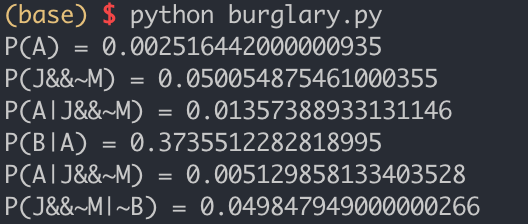
\includegraphics[width=10cm]{Pic/my_burglary.png}
\end{figure}


\subsection{Diagnosing}
\begin{lstlisting}[title=diagnosing.py]
from pomegranate import *
PatientAge = DiscreteDistribution({
    '0-30': 0.10,
    '31-65': 0.30,
    '65+': 0.60
})
CTScanResult = DiscreteDistribution({
    'Ischemic Stroke': 0.7,
    'Hemmorraghic Stroke': 0.3
})
MRIScanResult = DiscreteDistribution({
    'Ischemic Stroke': 0.7,
    'Hemmorraghic Stroke': 0.3
})
Anticoagulants = DiscreteDistribution({
    'Used': 0.5,
    'Not used': 0.5
})

StrokeType = ConditionalProbabilityTable([
    ['Ischemic Stroke','Ischemic Stroke','Ischemic Stroke',0.8],
    ['Ischemic Stroke','Hemmorraghic Stroke','Ischemic Stroke',0.5],  
    ['Hemmorraghic Stroke','Ischemic Stroke','Ischemic Stroke',0.5],
    ['Hemmorraghic Stroke','Hemmorraghic Stroke','Ischemic Stroke',0], 

    ['Ischemic Stroke','Ischemic Stroke','Hemmorraghic Stroke',0],
    ['Ischemic Stroke','Hemmorraghic Stroke','Hemmorraghic Stroke',0.4], 
    ['Hemmorraghic Stroke','Ischemic Stroke','Hemmorraghic Stroke',0.4],
    ['Hemmorraghic Stroke','Hemmorraghic Stroke','Hemmorraghic Stroke',0.9],

    ['Ischemic Stroke','Ischemic Stroke','Stroke Mimic',0.2],
    ['Ischemic Stroke','Hemmorraghic Stroke','Stroke Mimic',0.1],    
    ['Hemmorraghic Stroke','Ischemic Stroke','Stroke Mimic',0.1],
    ['Hemmorraghic Stroke','Hemmorraghic Stroke','Stroke Mimic',0.1]
], [CTScanResult, MRIScanResult])

Mortality = ConditionalProbabilityTable([
    ['Ischemic Stroke', 'Used', 'False',0.28],
    ['Hemmorraghic Stroke', 'Used', 'False',0.99],
    ['Stroke Mimic', 'Used', 'False',0.1],
    ['Ischemic Stroke','Not used', 'False',0.56],
    ['Hemmorraghic Stroke', 'Not used', 'False',0.58],
    ['Stroke Mimic', 'Not used', 'False',0.05],

    ['Ischemic Stroke',  'Used' ,'True',0.72],
    ['Hemmorraghic Stroke', 'Used', 'True',0.01],
    ['Stroke Mimic', 'Used', 'True',0.9],
    ['Ischemic Stroke',  'Not used' ,'True',0.44],
    ['Hemmorraghic Stroke', 'Not used', 'True',0.42 ],
    ['Stroke Mimic', 'Not used', 'True',0.95]
], [StrokeType, Anticoagulants])

Disability = ConditionalProbabilityTable([
    ['Ischemic Stroke',   '0-30','Negligible', 0.80],
    ['Hemmorraghic Stroke', '0-30','Negligible', 0.70],
    ['Stroke Mimic',        '0-30', 'Negligible',0.9],
    ['Ischemic Stroke',     '31-65','Negligible', 0.60],
    ['Hemmorraghic Stroke', '31-65','Negligible', 0.50],
    ['Stroke Mimic',        '31-65', 'Negligible',0.4],
    ['Ischemic Stroke',     '65+'  , 'Negligible',0.30],
    ['Hemmorraghic Stroke', '65+'  , 'Negligible',0.20],
    ['Stroke Mimic',        '65+'  , 'Negligible',0.1],

    ['Ischemic Stroke',     '0-30' ,'Moderate',0.1],
    ['Hemmorraghic Stroke', '0-30' ,'Moderate',0.2],
    ['Stroke Mimic',        '0-30' ,'Moderate',0.05],
    ['Ischemic Stroke',     '31-65','Moderate',0.3],
    ['Hemmorraghic Stroke', '31-65','Moderate',0.4],
    ['Stroke Mimic',        '31-65','Moderate',0.3],
    ['Ischemic Stroke',     '65+'  ,'Moderate',0.4],
    ['Hemmorraghic Stroke', '65+'  ,'Moderate',0.2],
    ['Stroke Mimic',        '65+'  ,'Moderate',0.1],

    ['Ischemic Stroke',     '0-30' ,'Severe',0.1],
    ['Hemmorraghic Stroke', '0-30' ,'Severe',0.1],
    ['Stroke Mimic',        '0-30' ,'Severe',0.05],
    ['Ischemic Stroke',     '31-65','Severe',0.1],
    ['Hemmorraghic Stroke', '31-65','Severe',0.1],
    ['Stroke Mimic',        '31-65','Severe',0.3],
    ['Ischemic Stroke',     '65+'  ,'Severe',0.3],
    ['Hemmorraghic Stroke', '65+'  ,'Severe',0.6],
    ['Stroke Mimic',        '65+'  ,'Severe',0.8]
], [StrokeType, PatientAge])

sPA = State(PatientAge, name='PatientAge')         # 0
sCT = State(CTScanResult, name='CTScanResult')     # 1
sMR = State(MRIScanResult, name='MRIScanResult')   # 2
sAN = State(Anticoagulants, name='Anticoagulants') # 3
sDI = State(Disability, name='Disability')         # 4
sST = State(StrokeType, name='StrokeType')         # 5
sMO = State(Mortality, name='Mortality')           # 6

model = BayesianNetwork('Diagnosing')
model.add_states(sPA, sCT, sMR, sAN, sDI, sST, sMO)
model.add_transition(sPA, sDI)
model.add_transition(sCT, sST)
model.add_transition(sMR, sST)
model.add_transition(sAN, sMO)
model.add_transition(sST, sDI)
model.add_transition(sST, sMO)
model.bake()

result1 = model.predict_proba({'PatientAge': '31-65', 'CTScanResult': 'Ischemic Stroke'})[6].parameters[0]['True']
print('p1 = {:.5f}'.format(result1))
result2 = model.predict_proba({'PatientAge': '65+', 'MRIScanResult': 'Hemmorraghic Stroke'})[4].parameters[0]['Moderate']
print('p2 = {:.2f}'.format(result2))
result3 = model.predict_proba({'PatientAge': '65+', 'CTScanResult': 'Hemmorraghic Stroke', 'MRIScanResult': 'Ischemic Stroke'})[5].parameters[0]['Stroke Mimic']
print('p3 = {:.1f}'.format(result3))
result4 = model.predict_proba({'PatientAge': '0-30'})[3].parameters[0]['Not used']
print('p4 = {:.1f}'.format(result4))
\end{lstlisting}

\begin{figure}[ht]
\centering
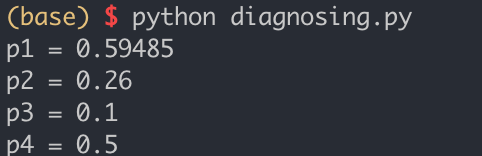
\includegraphics[width=10cm]{Pic/my_diagnosing.png}
\end{figure}

%\clearpage
%\bibliography{E:/Papers/LiuLab}
%\bibliographystyle{apalike}
\end{document} 
%%% Local Variables:
%%% mode: latex
%%% TeX-master: t
%%% End:
